\chapter{Supplementary material for \cref{chapter:SD433_Spectrum}}
\label{app:chap_spectrum}
\chaptermark{SD-433 supplementary material}

\section{Simple-power-law fit}
\label{app:sd433_powerlaw}

The simple-power-law hypothesis is tested using the same event counts, migration matrix and fit interval as the nominal \sd{433} spectrum analysis.
\Cref{fig:sd433_powerlaw_fit} compares the nominal unfolded spectrum with the fitted simple-power-law and broken-power-law functions.
The simple-power-law fit to the measured event counts gives $D/\mathrm{dof}=\SDFourThreeThreePowerLawDeviance/\SDFourThreeThreePowerLawDof$ and $p=\SDFourThreeThreePowerLawPValue$.
The broken-power-law prediction uses the nominal fit with $\omega_{01}=0.05$.

\begin{figure}[!htbp]
    \centering
    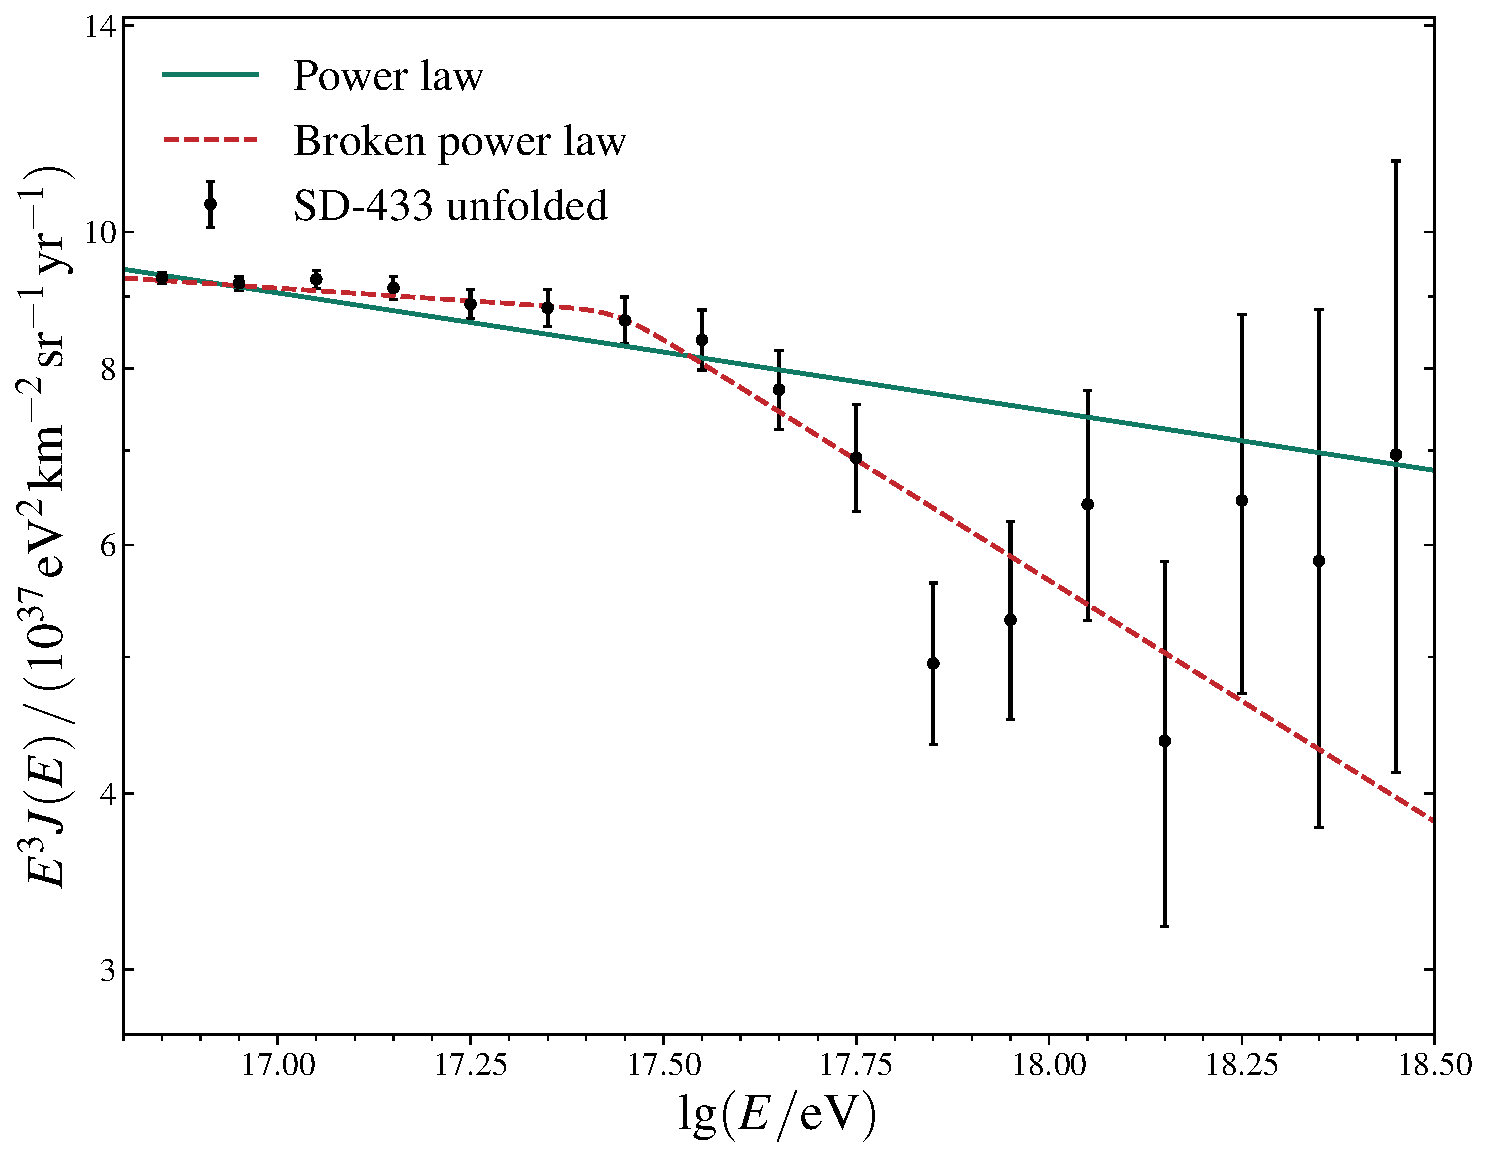
\includegraphics[width=0.78\linewidth]{figures/chapter_spectrum/sd433_power_law_test.pdf}
    \caption[Simple-power-law test of the SD-433 spectrum]{Simple-power-law fit to the \sd{433} spectrum.
    The upper panel shows the nominal unfolded spectrum multiplied by $E^3$ and the fitted simple-power-law (solid) and nominal broken-power-law (dashed) functions before folding with the detector response.
    The lower panel shows relative differences with respect to the fitted simple power law; the dashed curve gives the broken-power-law comparison.
    Points use the nominal unfolding and show statistical uncertainties.
    The quoted deviance and $p$-value are calculated from the forward-folded fit to measured event counts over $16.8<\lg(E/\mathrm{eV})<18.5$, rather than from the displayed unfolded residuals.}
    \label{fig:sd433_powerlaw_fit}
\end{figure}

\clearpage
\section{Energy-scale variations}
\label{app:sd433_energy_scale}

\Cref{fig:sd433_energy_scale_spectra} shows the unfolded spectra obtained after shifting all reconstructed event energies coherently by $-14\%$ and $+14\%$.
The detector response is kept fixed, and the forward-folding fit and unfolding are repeated for each shifted event distribution.
The corresponding fitted parameters and relative flux variations are discussed in \cref{sec:systematics}.

\begin{figure}[htbp]
    \centering
    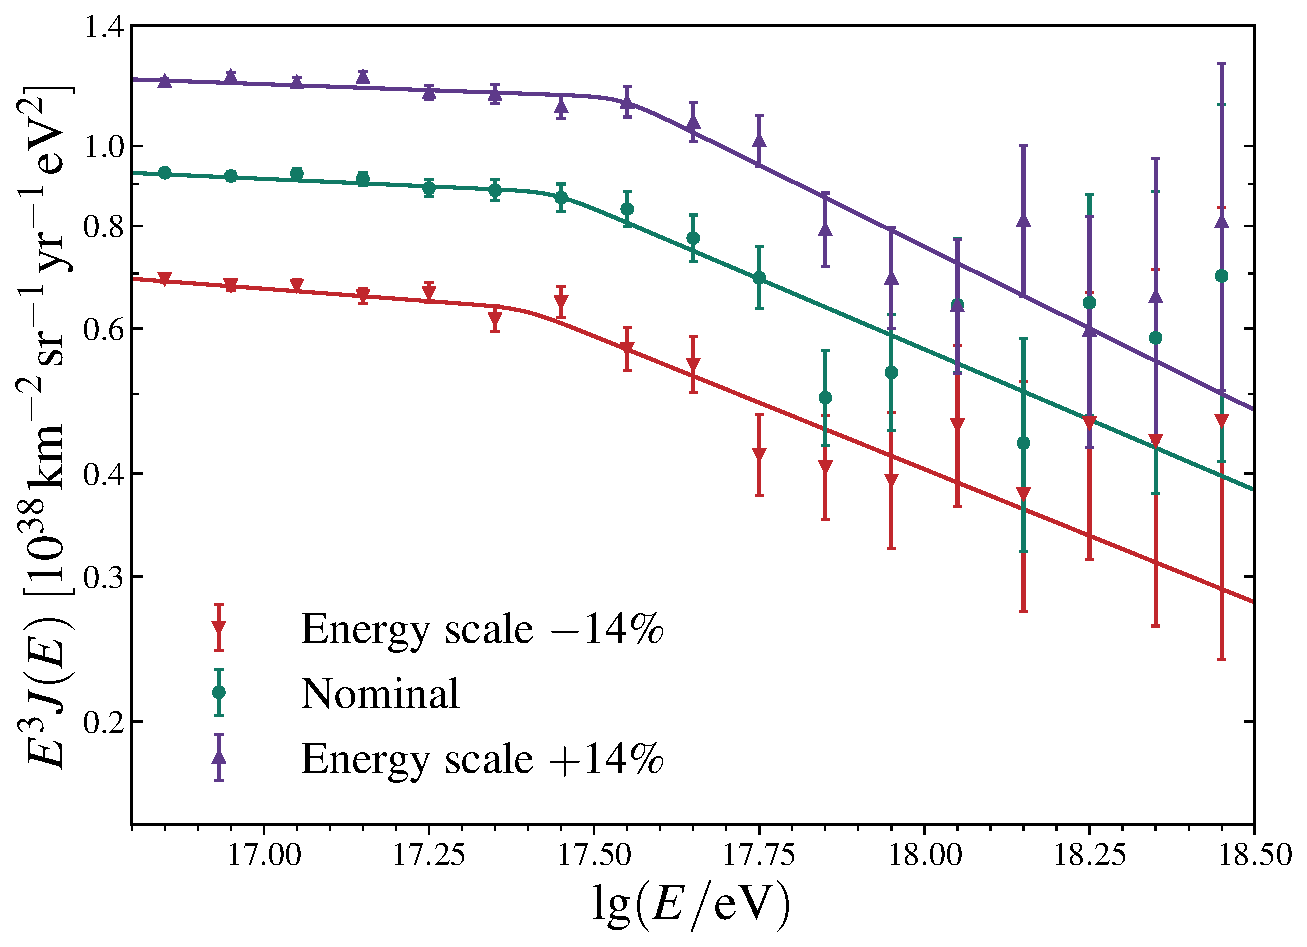
\includegraphics[width=\linewidth]{figures/chapter_spectrum/sd433_energy_scale_unfolded_spectra.pdf}
    \caption[SD-433 unfolded spectra with shifted energy scales]{Unfolded \sd{433} spectra for the nominal energy scale and coherent shifts of $-14\%$ and $+14\%$.
    Points show the unfolded fluxes with statistical uncertainties; curves show the corresponding forward-folding fits.
    The migration matrix is unchanged, and all fits use $16.8<\lg(E/\mathrm{eV})<18.5$ and $\omega_{01}=0.05$.}
    \label{fig:sd433_energy_scale_spectra}
\end{figure}

\clearpage
\section{Energy-resolution variations}
\label{app:sd433_resolution}

The resolution study varies $R_{\mathrm{sh}}$ and $R_0$ simultaneously by their respective $1\sigma$ uncertainties, keeping the other response components unchanged.
The nominal values are $R_{\mathrm{sh}}=0.09$ and $R_0=0.21/\sqrt{3}$, with an uncertainty of $0.01$ assigned to each parameter.
For each variation, the migration matrix is recalculated and the spectrum is refitted with $\omega_{01}=0.05$ over the nominal energy interval.
\Cref{fig:sd433_resolution_spectra,fig:sd433_resolution_fit_parameters} show the resulting spectra and fitted parameters.

\begin{figure}[htbp]
    \centering
    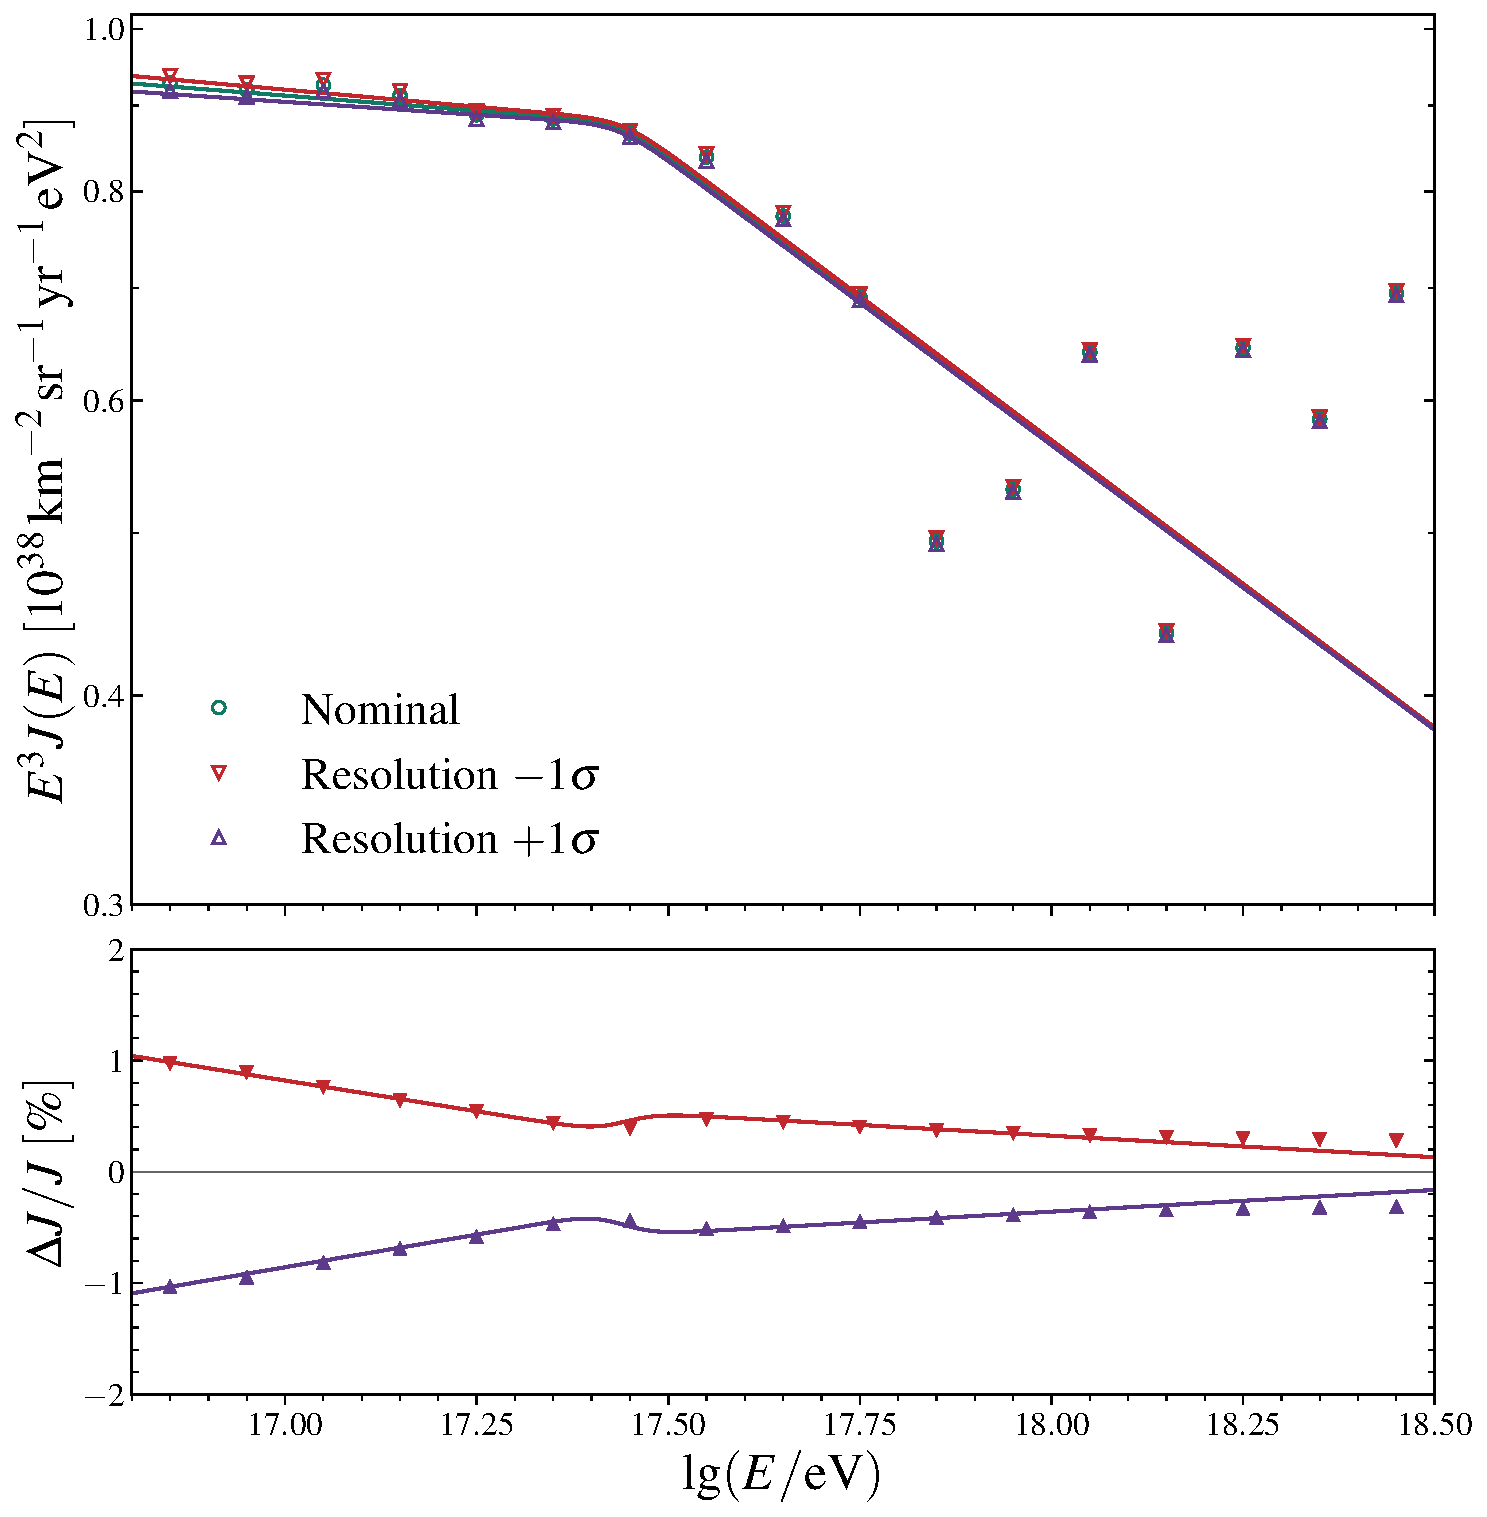
\includegraphics[width=0.93\linewidth]{figures/chapter_spectrum/sd433_resolution_unfolded_spectra.pdf}
    \caption[SD-433 spectra with varied energy resolution]{Effect of the energy-resolution uncertainty on the unfolded \sd{433} spectrum.
    Both resolution parameters are shifted simultaneously by their respective one-standard-deviation uncertainties.
    Upper panel: unfolded spectra (points) and fitted models (curves), shown with a logarithmic flux axis.
    Lower panel: relative differences with respect to the corresponding nominal unfolded fluxes and fitted model.
    Statistical uncertainties are omitted to show the small changes.}
    \label{fig:sd433_resolution_spectra}
\end{figure}

\begin{figure}[p]
    \centering
    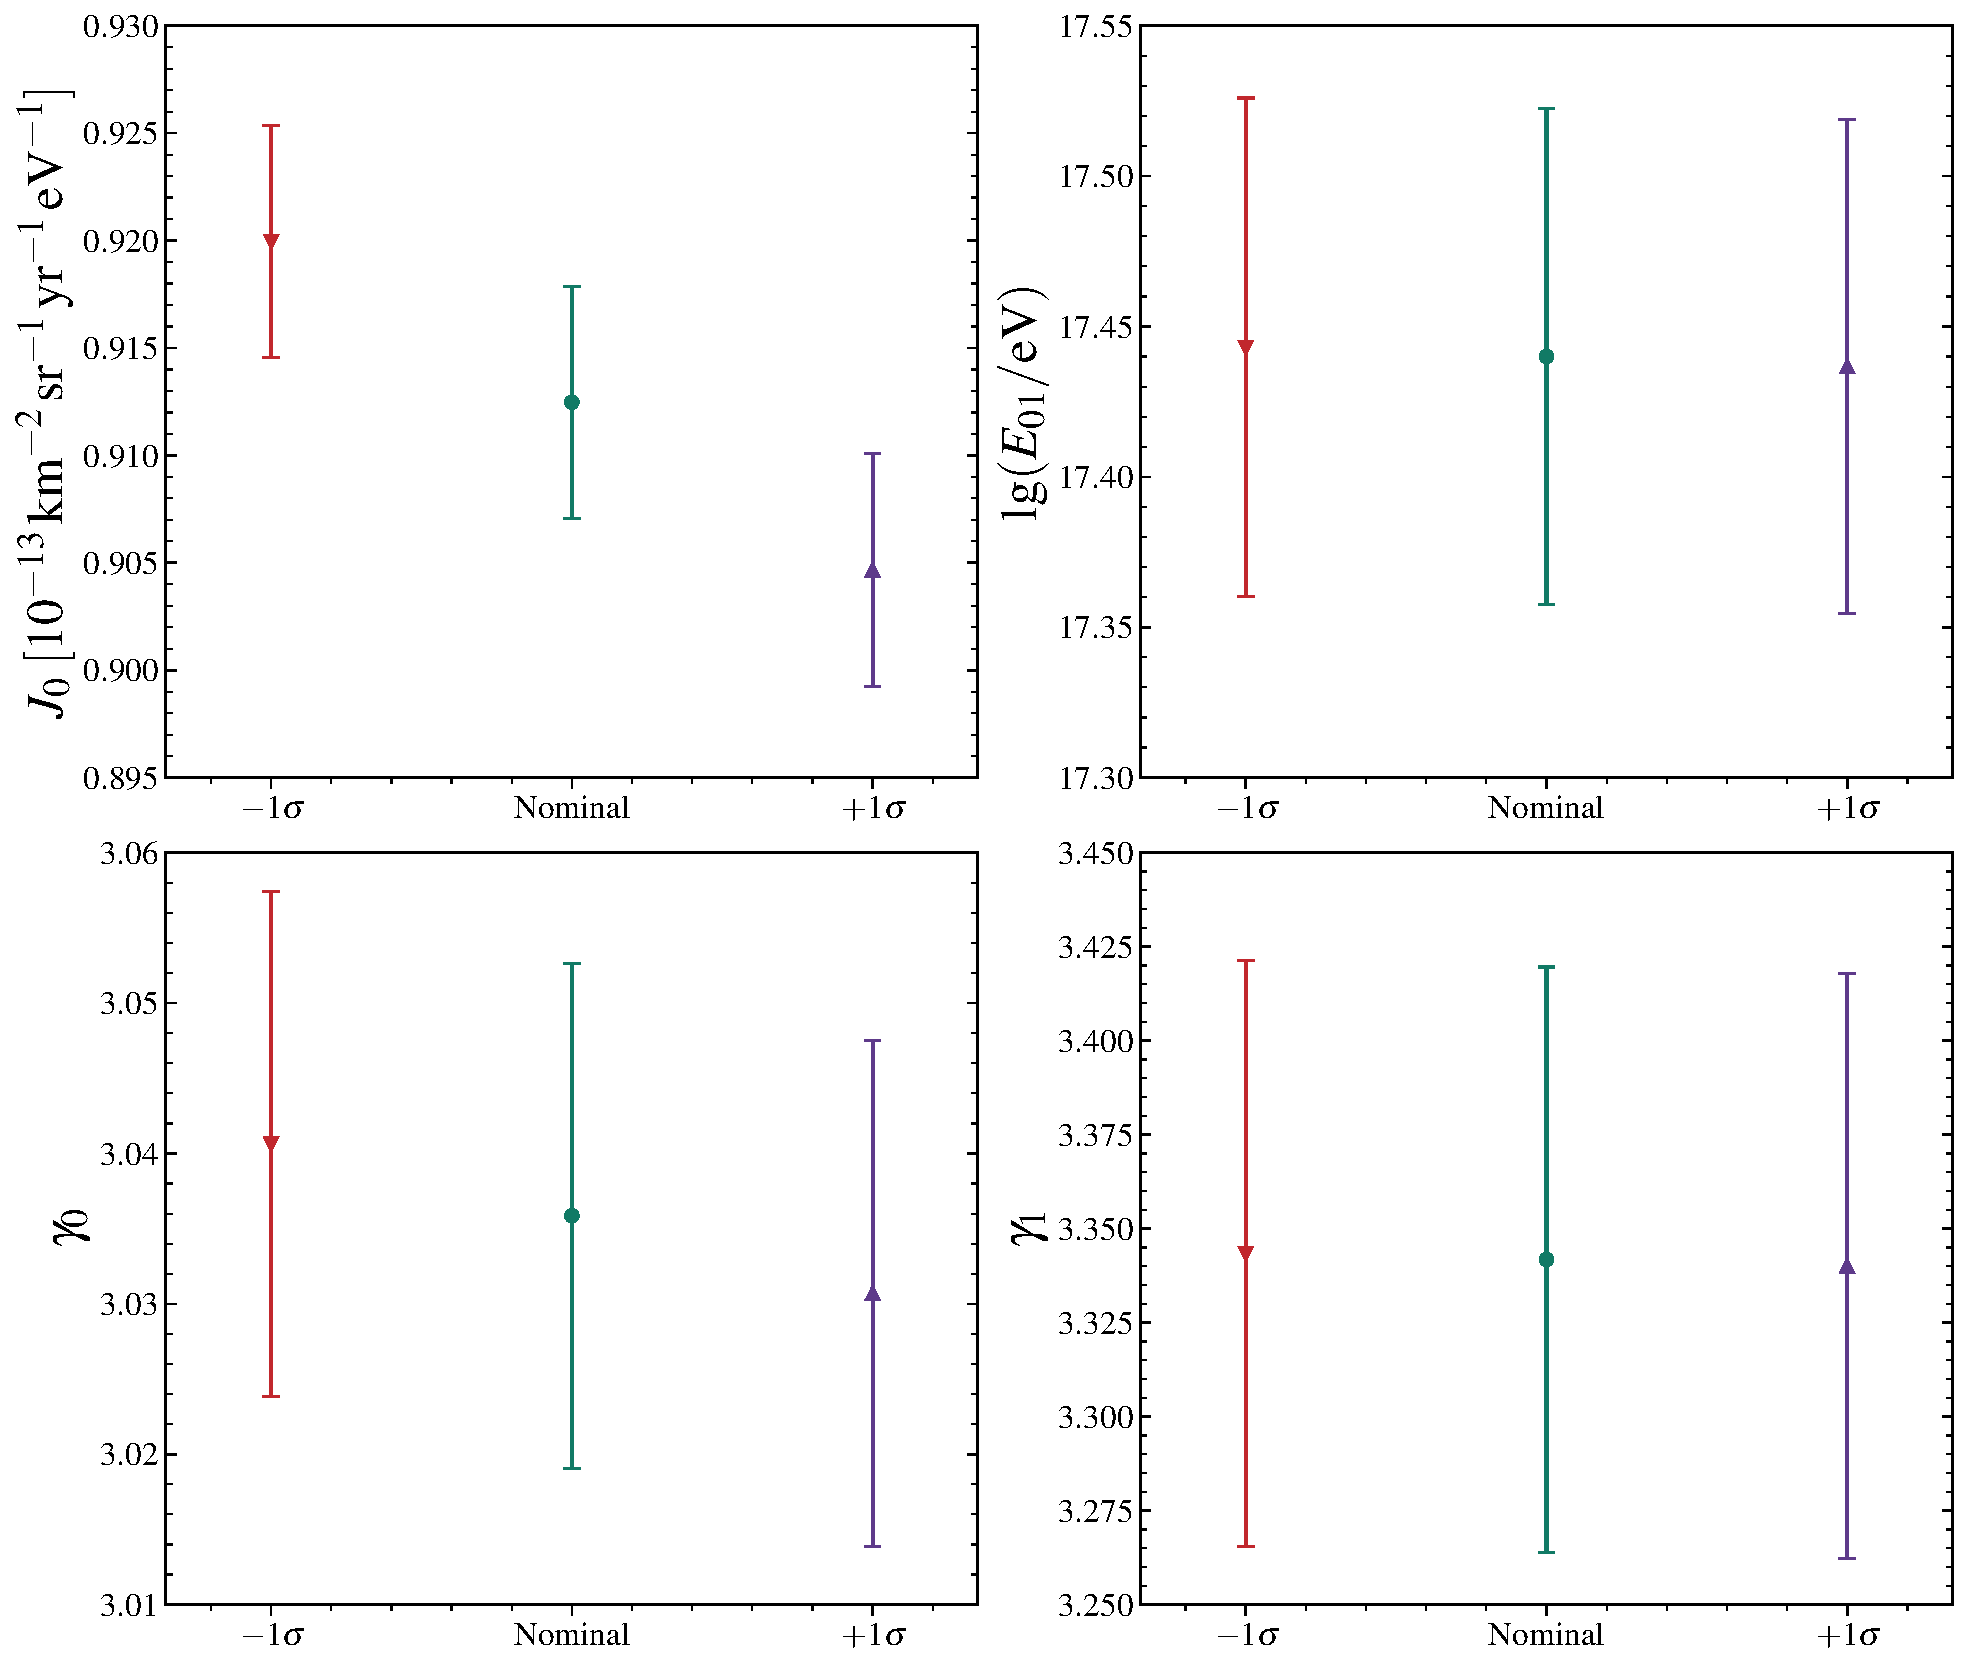
\includegraphics[width=\linewidth]{figures/chapter_spectrum/sd433_resolution_fit_parameters.pdf}
    \caption[SD-433 fitted parameters with varied energy resolution]{Fitted \sd{433} spectral parameters for the nominal resolution and simultaneous downward and upward one-standard-deviation shifts of its parameters.
    Error bars show statistical fit uncertainties.
    The transition width is fixed to $\omega_{01}=0.05$ in all three fits.}
    \label{fig:sd433_resolution_fit_parameters}
\end{figure}
